\documentclass[12pt]{scrartcl}

\usepackage[sexy]{evan}
\usepackage{packs}

%%%%%%%%%%%%%%%%%%%%%%%%%%%%%%%%%%%%%%%%%%%%%%%%%%%%%%%%%%%%%%%%%%%%%%%

\title{LaTeX Template}
\author{Avigyan Chakraborty}
\date{Last Updated: \today}

\begin{document}

\maketitle

\tableofcontents

\pagebreak

\section{Environments}

This is some \bluebf{bold text} with the dark blue colour.

\begin{definition}
[Name]
This is a Definition.
\end{definition}

\begin{theorem}
[Name]
This is a Theorem.
\end{theorem}

\begin{lemma}
[Name]
This is a Lemma.
\end{lemma}

\begin{corollary}
[Name]
This is a Corollary.
\end{corollary}

\begin{proposition}
[Name]
This is a Proposition.
\end{proposition}

\begin{assume}
[Name]
This is an Assumption.
\end{assume}

\begin{conjecture}
[Name]
This is a Conjecture.
\end{conjecture}

\begin{fact}
[Name]
This is a Fact.
\end{fact}

\begin{ques}
[Name]
This is a Question.
\end{ques}

\begin{answer}
[Name]
This is an Answer.
\end{answer}

\begin{exercise}
[Name]
This is an Exercise.
\end{exercise}

\begin{problem}
[Name]
This is a Problem.
\end{problem}

\begin{algorithm}
[Name]
This is an Algorithm.
\end{algorithm}

\begin{claim}
[Name]
This is a Claim.
\end{claim}

\begin{proof}
This is a Proof.
\end{proof}

\begin{example}
[Name]
This is an Example.
\end{example}

\begin{soln}
This is a Solution.
\end{soln}

\begin{remark}
[Name]
This is a Remark.
\end{remark}

\section{Fitting images perfectly}

So, fitting images has ever been a hectic problem for me just because I am an idiot. Here is literally the easiest way to fit images lol. You can use [scale=*] for custom scaling to the figures if necessary.

\begin{figure}[h]
    \centering
    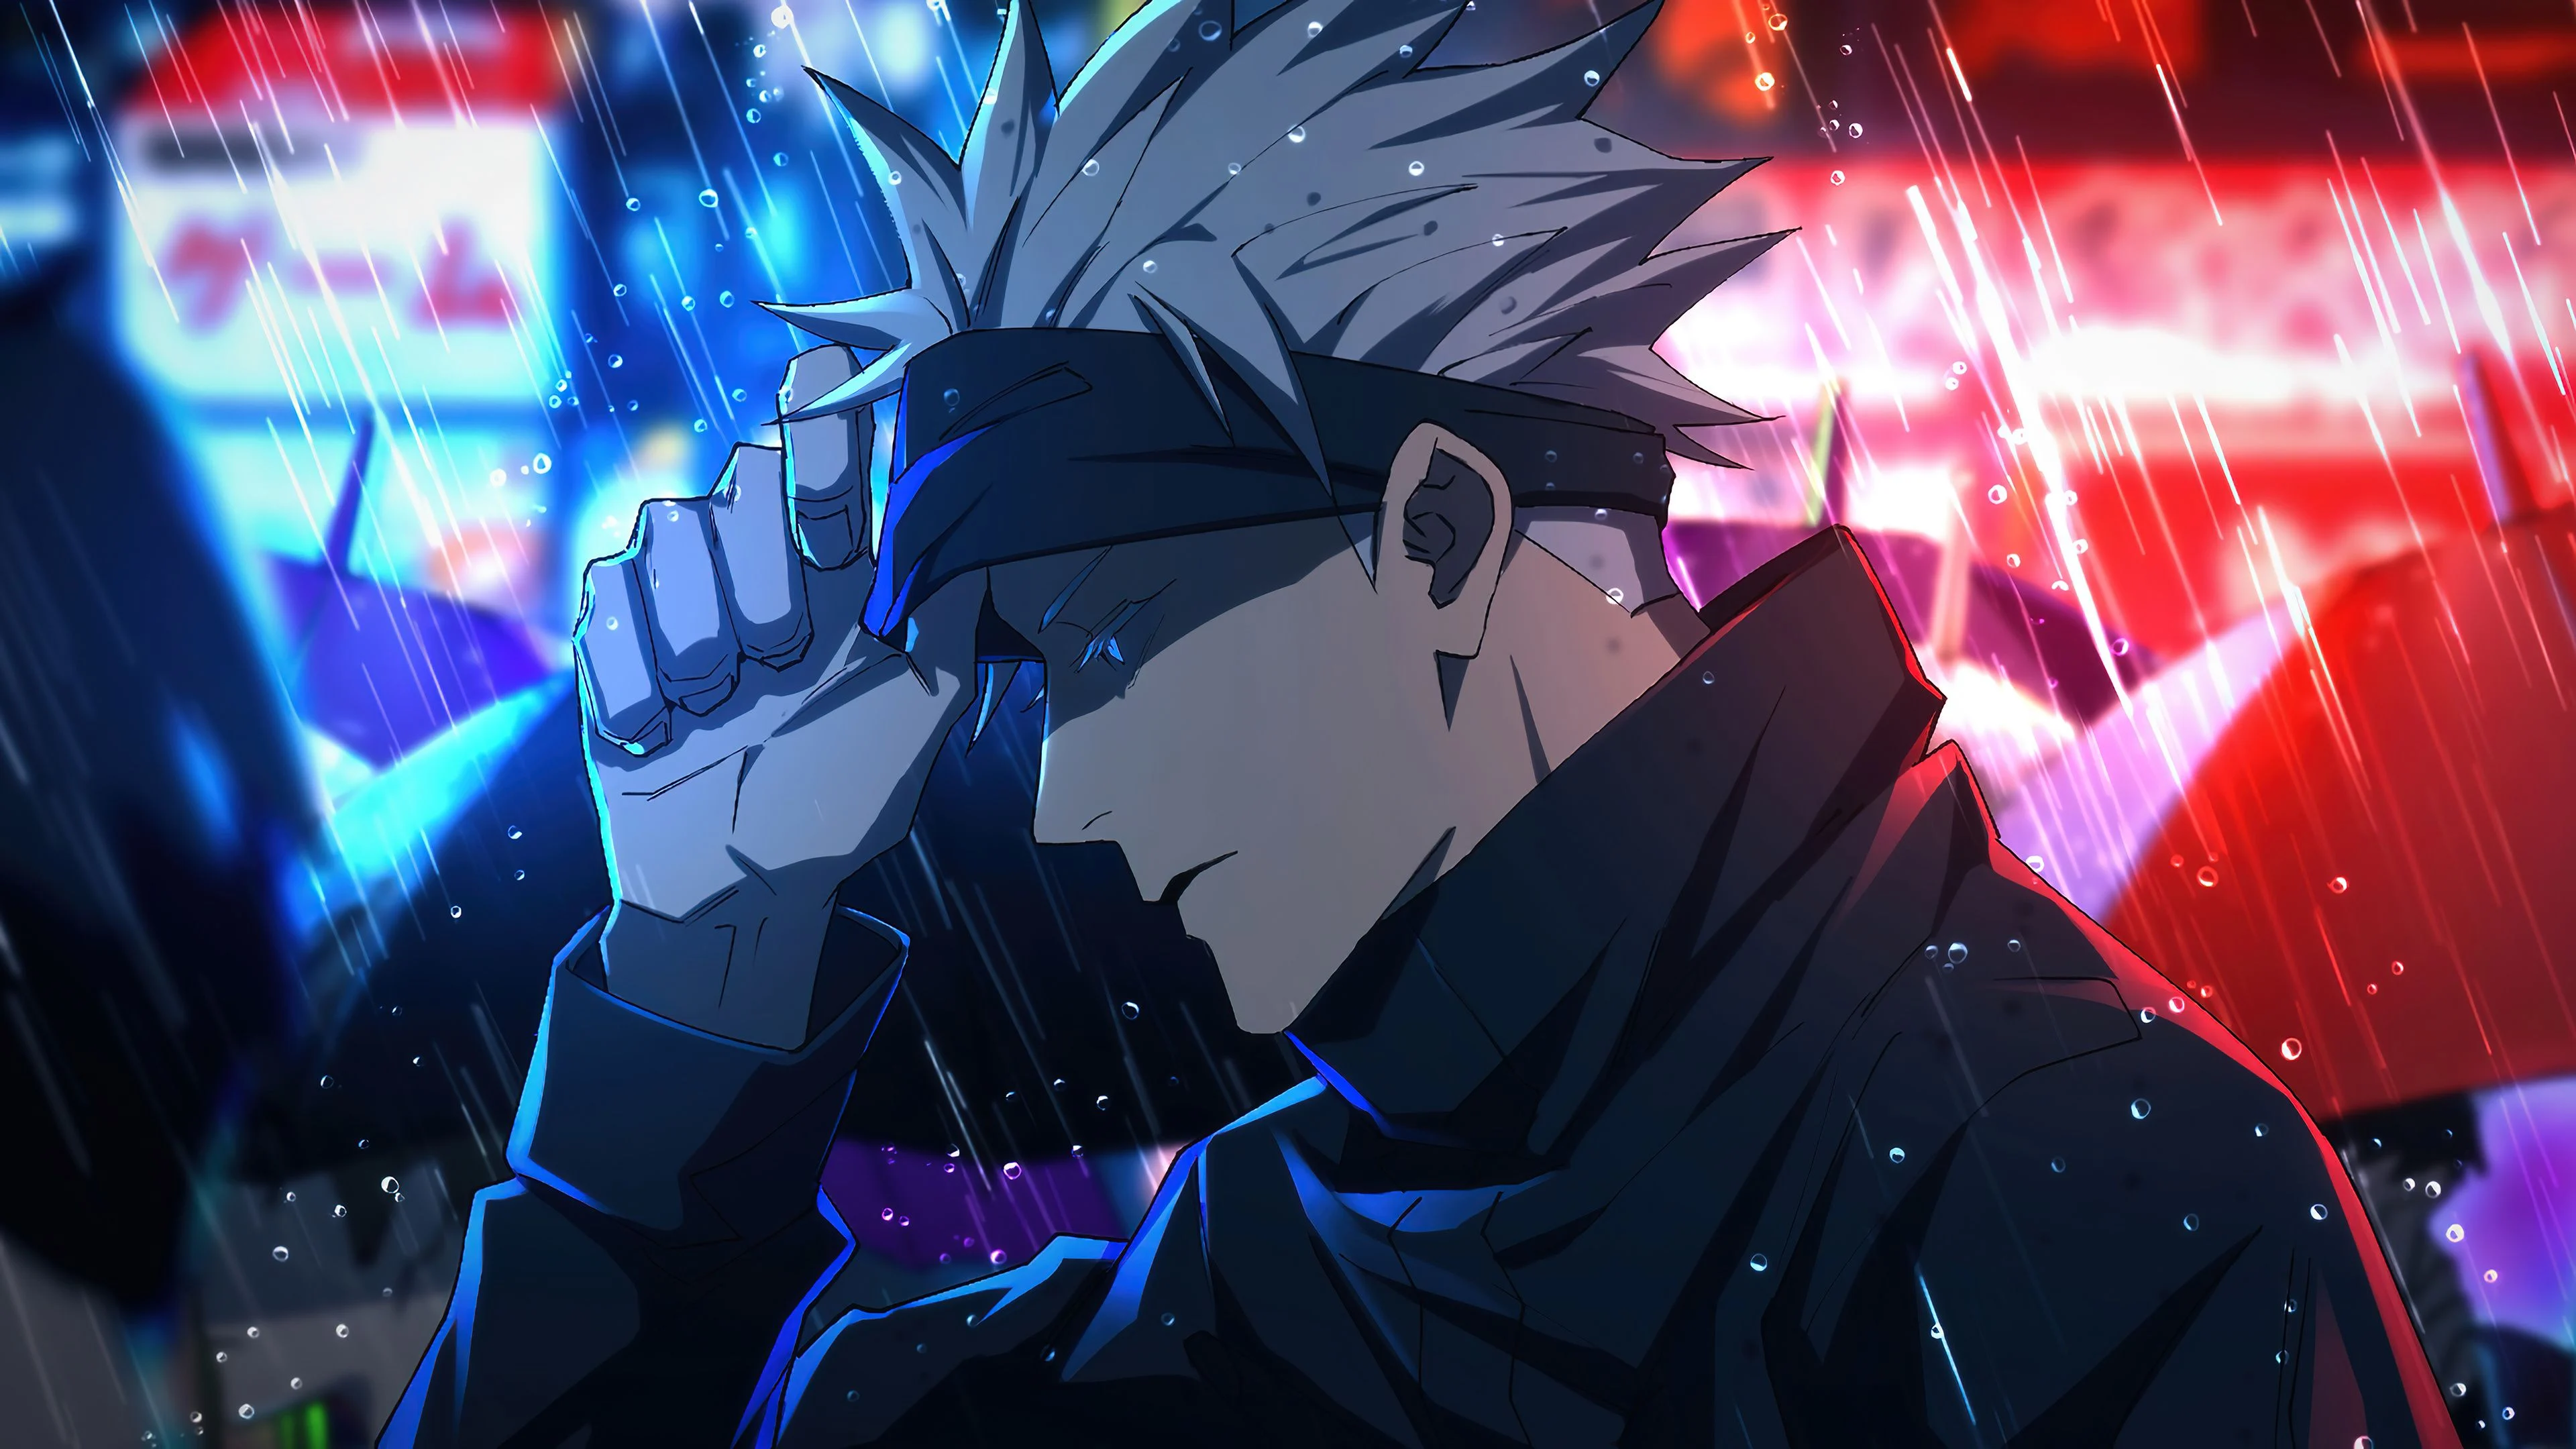
\includegraphics[width=\textwidth,keepaspectratio]{images/gojo_pfp.png}
    % height=\textheight does what it's expected to do similarly as well
    \caption{Gojo cool asf 4K Wallpaper}
    \label{gojo4kwallpaper}
\end{figure}

\end{document}
